\section{Adaptive Mesh Refinement test}
There are 10720 cells: 10482 quadrilaterals, 236 pentagons, and 2 hexagons 
for a total of 43120 degrees of freedom. The distribution is given by:
\begin{figure}[H]
  \centering
  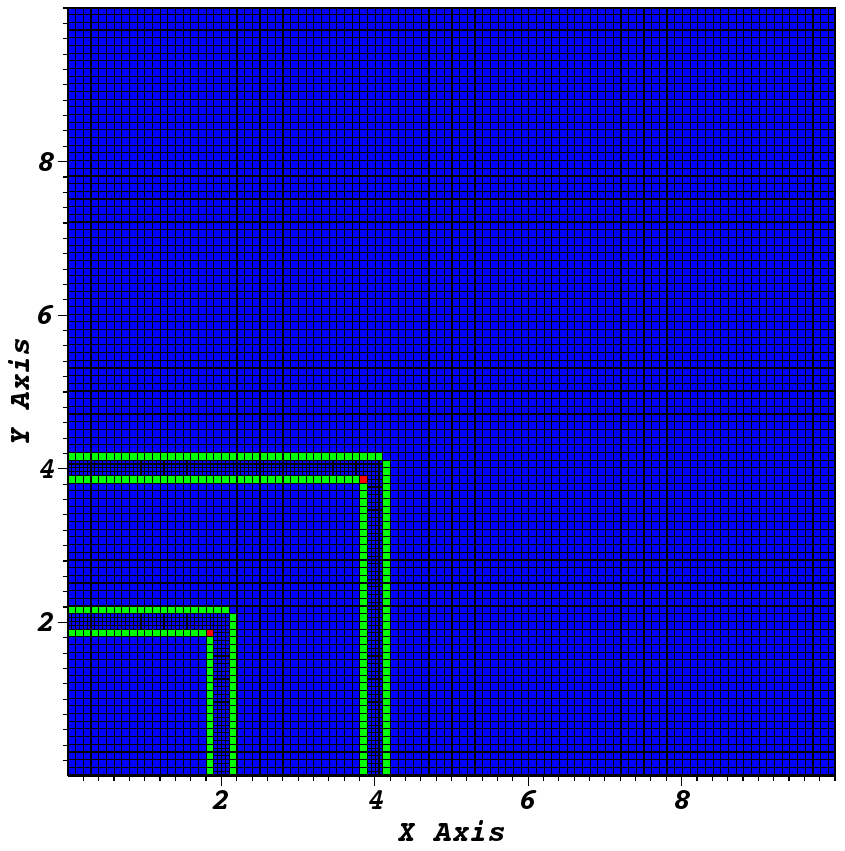
\includegraphics[width=4cm]{polygon_amr}
  \caption{Polygons distribution}
\end{figure}
\begin{itemize}
  \item Blue cells are quadrilaterals.
  \item Green cells are pentagons.
  \item Red cells are hexagons.
\end{itemize}
The domain is composed if three zones:
\begin{description}
  \item[Green zone:] $\Sigma_t=1cm^{-1}$, $\Sigma_s=0.9cm^{-1}$,
    source=$1cm^{-3}s^{-1}$
  \item[Red zone:] $\Sigma_t=1.5cm^{-1}$, $\Sigma_s=1.44cm^{-1}$, no source
  \item[Blue zone:] $\Sigma_t=1cm^{-1}$, $\Sigma_s=0.3cm^{-1}$, no source
\end{description}
We use a $S_{16}$ GLC quadrature, with SI, tolerance is $10^{-8}$, PWLD,
bottom and left boundaries are reflective, right and top boundaries vacuum.
\begin{table}[H]
  \caption{Comparison of preconditioners on AMR mesh.}
  \begin{centering}
    \begin{tabular}{|c|c|c|c|c|c|c|}
      \hline
       & No-DSA & CG & PCG-SGS & PCG-MLU & PCG-MLM & AGMG \\
      \hline
      SI iter    & 184     & 19      &
      Prec (s)   & NA      & NA      &
      MIP (s)    & NA      & 48.1908 &
      CG iter    & NA      & 11300   & 4734
      Total (s)  & 802.985 & 138.825 &
    \end{tabular}
  \end{centering}
\end{table}
